\begin{figure*}
  \begin{center}
    \begin{tabular}{c}
      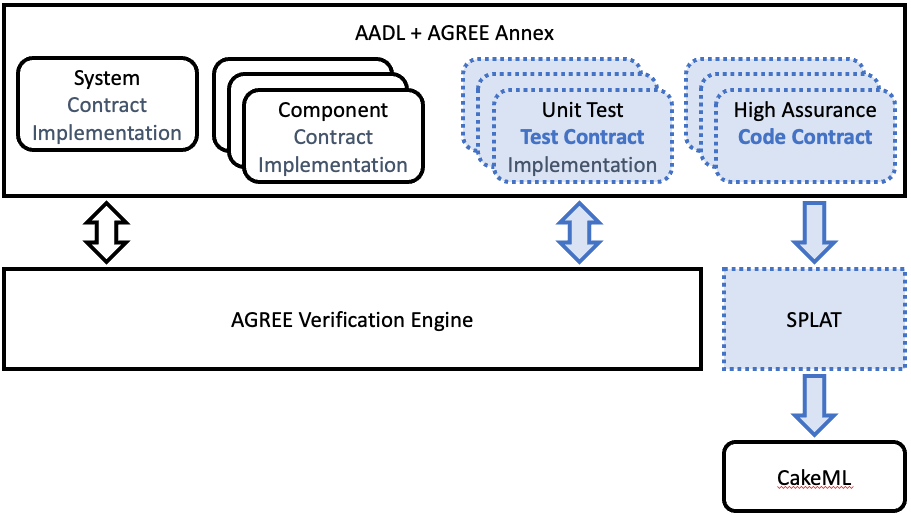
\includegraphics[width=0.8\textwidth]{flowchart.png} \\
    \end{tabular}
  \end{center}
\caption{A simplified illustration of the \brfcs\ toolkit with shaded portions being the contributions presented here.}
\label{fig:flowchart}
\end{figure*}

\begin{figure*}
	\begin{center}
	  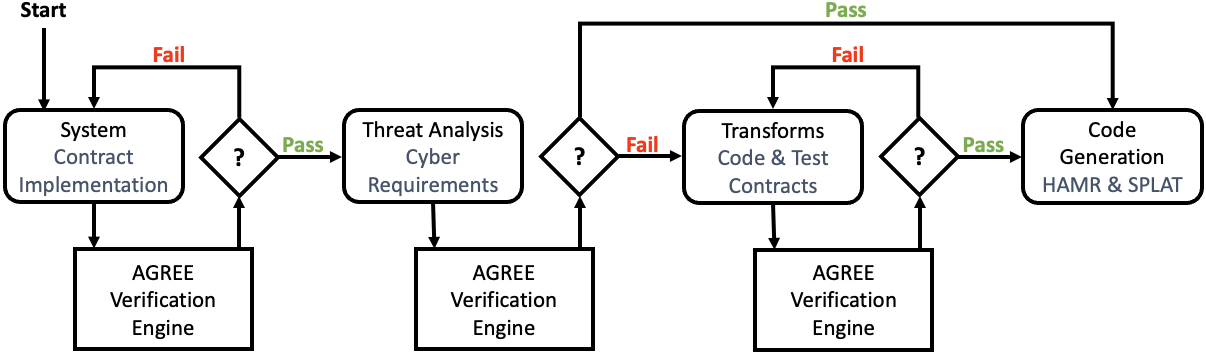
\includegraphics[width=\textwidth]{./figs/workflow.png}
  	\end{center}
	\caption{The general workflow for \brfcs.}
	\label{fig:workflow}
\end{figure*}

The \brfcs\ OSATE environment provides designers with workflow and tool support for developing products with
inherent cyber-resiliency.
%
\figref{fig:flowchart} is a simplified illustration of the toolkit that omits tooling outside of our contributions discussed here (see \cite{dcrypps2019,gearcase2020,resolute-destion,attestation-copland,awas,hamr,sel4-sosp09, sel4-tocs14, sel4-cacm18} for other aspects of \brfcs).  
%
\newjunk{
The shaded boxes represent our contribution: test contracts, code contracts, and SPLAT synthesis.
The unshaded boxes are the existing tools that provide the foundation for our contributions.}

\newjunk{
The intended \brfcs\ workflow is in \figref{fig:workflow}.
%
The workflow starts with a behavioral description of the system and its components on the left.
%
These descriptions are contracts that assume properties on inputs and guarantee properties on outputs when the input assumptions hold.
Once \agr\ verifies the system contract composition, the workflow moves right to the threat analysis, and the contracts of the system and components are modified to reflect that analysis.
%
If \agr\ verifies the system contract composition with the changes from the threat analysis, then the workflow moves to the far right for code generation.
%
Otherwise it moves immediate right to transforms. 
Here the designer inserts high-assurance components such as filters and monitors, with their accompanying code contracts, until \agr\ verifies the new system composition to be cyber-resilient to the indicated threats.
%
Once \agr\ verifies the new system composition, the workflow moves to code generation, where \splt\ synthesizes implementations for the inserted high-assurance components from their corresponding code contracts.
}

\newjunk{
We use this section to explain both figures in more detail through an example.
%
The example is a UAV system for remote monitoring, and it is loosely based on
the case study in \secref{sec:case-study}.  
%
The source for the example is at \cite{repo}.
%
The intent of the UAV system is to receive a mission from the ground station, plan a path to fly that mission from its current location, and then fly the planned path updating the ground station along the way.
%
The system must by cyber-resilient and actively protect itself from malicious actors to ensure it is sending accurate monitoring information back to the ground station and that it actually flies the intended mission.
}

\subsection{System and Component Contract Implementation}

\begin{figure*}[h]
  \begin{center}
    \begin{tabular}{c}
      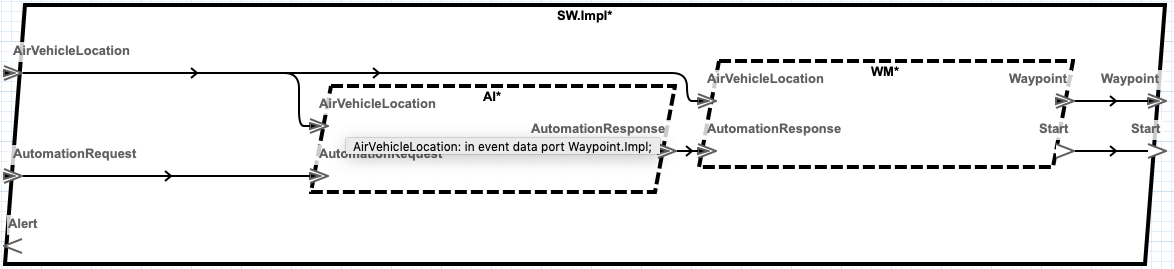
\includegraphics[width=\textwidth]{example.png}
    \end{tabular}
  \end{center}
\caption{Initial design for an automated UAV route planning system.}
\label{fig:example}
\end{figure*}

\begin{figure}
  \begin{center}
    \begin{tabular}{c}
      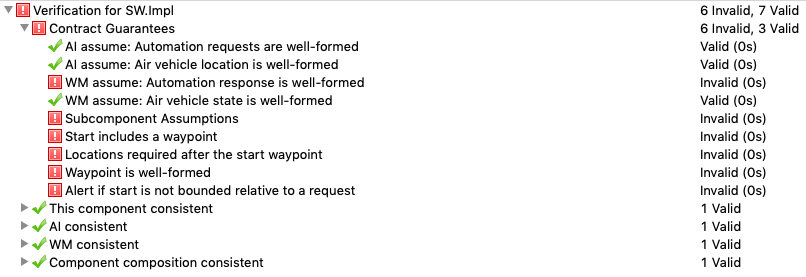
\includegraphics[width=1\columnwidth]{example-certificate.png} \\
    \end{tabular}
  \end{center}
\caption{\agr\ failure certificate for initial design.}
\label{fig:example-certificate}
\end{figure}

\newjunk{
We focus on the software system for the UAV in this example.
%
The AADL architecture model for that system consists of two components as shown in \figref{fig:example}.
The first is the component for the automatic path planning for a mission (AI). 
And the second is the component to meter the flight path waypoints to the actual UAV flight controller (WM).
}

From time to time, SW receives a message on the \texttt{AutomationRequest} input,
forwarding it to the AI. The function of AI is to
compute the flight path (a list of waypoints) for the UAV, outputting
the resulting \emph{mission command} on \texttt{AutomationResponse}.
The WM receives the mission command from AI and
starts the UAV flying the mission by putting an \emph{event} on the
\texttt{Start} output port, continuing to issue waypoints to the UAV
flight controller on the \texttt{Waypoint} port as the UAV location
updates with messages on \texttt{AirVehicleLocation}.
%%An event is repeatedly generated on \texttt{Alert} if there is no
%%mission command from a request.
The AI component is third-party
software and WM is a legacy component.

%% that cannot be modified so it critically relies on
%% assumptions about its input behavior to guarantee its intended output
%% behavior.

The expected behavior of the SW system, and the components
implementing the system, are modeled with \agr\ contract
specifications as shown by the unshaded boxes in the top-left of \figref{fig:workflow}.
These contracts assume and guarantee the absence
of any malicious, or unspecified, component behavior.  More precisely,
the contract for SW assumes that its inputs are \emph{well-formed} and that
there is never more than one automation request pending at a time.
Well-formed generally refers to a syntactic restriction on
data at a port. For example, a waypoint is well-formed if it falls
within bounds for latitude, longitude, and altitude.  The guarantees
for SW ensure that
\begin{compactitem}
\item a start coincides with a new waypoint being output;
\item a start is within one cycle of an automation request and if not, then it persistently alerts;
\item new waypoints coincide with location updates; and
\item all outputs are well-formed.
\end{compactitem}

The contracts for the sub-components assume their inputs are
well-formed, and they guarantee their outputs are well-formed.  The AI
contract guarantees it only responds to automation requests and always
in the same cycle.  The legacy WM contract guarantees that
\begin{compactitem}
  \item it generates a start from a response from the AI and always in the same cycle;
  \item the start coincides with a waypoint; and
  \item any further waypoints coincide with location updates.
\end{compactitem}

\newjunk{
\figref{fig:workflow} shows the intent of this behavioral contract definition of the UAV software system on the left-side of the figure at the arrow marked start.
The \agr\ verification engine tries to prove if the component composition of the software system is correct. 
It is an iterative process where the designer updates contracts in the composition until \agr\ proves out the composition.
}
For our example, the initial specifications described above pass verification, meaning that the
contract composition of the components with the system satisfies all
component input assumptions and system output guarantees.
The \agr\ verification conditions, syntax and semantics, and the baseline contracts for the example are discussed in detail in \secref{sec:agree}. 
\newjunk{\figref{fig:sw} in that section is the \agr\ contract for SW.}

\subsection{Adding cyber requirements}

\newjunk{
Having passed \agr\ verification, the workflow in \figref{fig:workflow} proceeds to the threat analysis stage.
The UAV must actively protect itself from malicious actors, but to this point, the designers have only been focusing on its core functional behavior with little consideration for cyber-resilience.
}
%
A cyber-vulnerability analysis identifies the potential of a
supply chain attack through the AI route planner since its third-party.  Based on the analysis, the designer adds a requirement that the system must guard against malicious AI behavior.
This requirement is reflected in the component contracts by removing all output guarantees from the AI contract since that component is considered untrusted.
Without output guarantees, the AI component is able to output arbitrary events in the \agr\ verification analysis.

The output from that analysis is shown in \figref{fig:example-certificate}.  The red
exclamation points designate component assumptions or system output
guarantees that do not hold, and each failure comes with a
corresponding counter-example.  The first violation is that the mission command on \texttt{AutomationResponse} from
the AI to the WM is no longer guaranteed to be well-formed: \newjunk{the red exclamation point on \emph{WM assume: Automation responses are well-formed}.  The
consequence of that failing input assumption is that the WM outputs
are no longer guaranteed. For a contract, when an input assumption does not hold, then the output may be arbitrary.}
The now arbitrary output from the WM due to input assumption violations lead to the rest of the failures
in \figref{fig:example-certificate} as the WM provides the system
level outputs.

\begin{figure*}
  \begin{center}
    \begin{tabular}{c}
      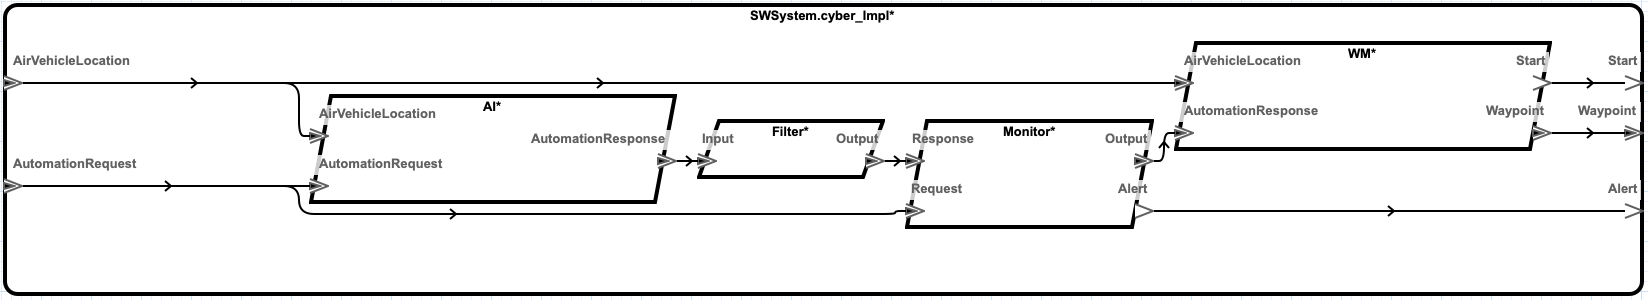
\includegraphics[width=2\columnwidth]{hardened.png}
    \end{tabular}
  \end{center}
  \caption{Cyber-hardened design for an automated UAV route planning system}
  \label{fig:hardened}
\end{figure*}

\begin{figure}
  \begin{center}
    \begin{tabular}{c}
      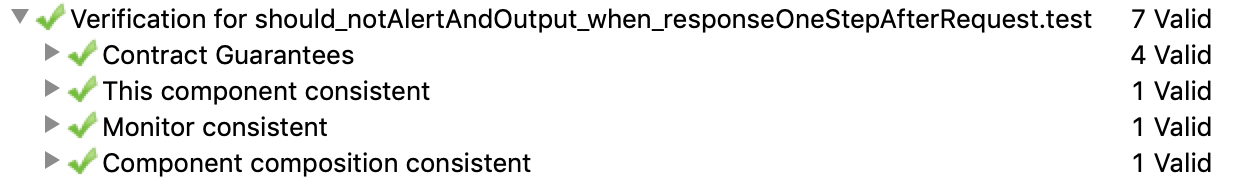
\includegraphics[width=\columnwidth]{agree-test-output.png} \\
      (a) \\ \\
      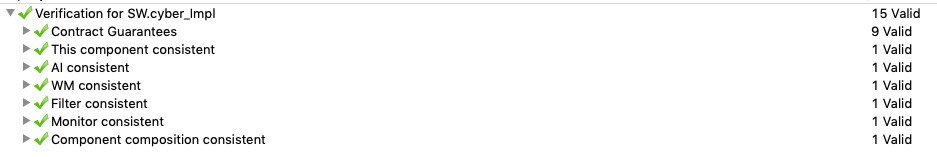
\includegraphics[width=\columnwidth]{hardened-certificate.png} \\
      (b)
    \end{tabular}
  \end{center}
  \caption{\agr\ verification certificates. (a) Test contract verification results. (b) Cyber-hardened design verification results.}
  \label{fig:hardened-certificate}
\end{figure}

\subsection{Adding high assurance components}

\newjunk{As \agr\ proves the system does not meet its cyber-requirements, the workflow moves to the right in \figref{fig:workflow} to the transforms box.}
Here is where the shaded regions in \figref{fig:flowchart} come into play.
The system designer now uses \brfcs\ to cyber-harden SW by inserting
high-assurance components in the form of a filter and a monitor, as
shown in \figref{fig:hardened}.
These are intended to mitigate and report any observed malicious behavior by AI.

A filter enforces an invariant over
each datum in the data stream by not forwarding input to its output if the invariant does not hold.
\brfcs\ generates an initial code contract for the filter which the designer completes by writing the invariant.
That invariant is usually based on the existing assumptions made by
downstream components that consume the filter output.
In this example, it is the well-formed property for the automation request.

A monitor captures a relation on data over time and is thus able
to reason about the temporal, and other invariant, properties of that data.  It raises
an alert if the specified properties are ever violated.
As with the filter, \brfcs\ generates an initial code contract that is completed by the designer.
In this example, that contract states that an
automation response can only be generated in conjunction with an
automation request; and further, that response must come with the
request or in the next step after the request.
Code contracts are discussed in detail in \secref{sec:code-contracts}.
\newjunk{
\figref{fig:filter} and \figref{fig:monitor} are the code contracts from that section for the high-assurance filter and monitor inserted into the original system as shown in \figref{fig:hardened}.}

Code contracts for high assurance components can be arbitrarily complex since they can have persistent state that evolves over time.
Test contracts allow the designer to validate code contract behavior with unit testing.
For example, one of the test contracts for the monitor is that when it sees an automation response one step after a request, then it should not alert, and it should pass the response downstream.
Test contracts are discussed in detail in \secref{sec:testing}.
\newjunk{
An example test from that section the the monitor in our example here is shown in \figref{fig:test}.
}

\newjunk{
As shown in \figref{fig:workflow}, making the system cyber-resilient is an iterative process of adding high-assurance components, writing their code contracts, testing those contracts with test contracts, and then seeing if they are sufficient to prove out the system.
}
Having completed such an iterative for our example system, 
the \agr\ analysis of the cyber-hardened implementation is shown in
\figref{fig:hardened-certificate}.
\figref{fig:hardened-certificate}(a) is the test contract results and \figref{fig:hardened-certificate}(b) is the hardened system composition.
Here \agr\ has generated high-level
evidence justifying the claim that the high-assurance components meet their intended purposes.
Having passed \agr\ verification, the high-assurance components are ready to be
synthesized.


\subsection{Synthesizing code from code contracts}

\newjunk{
As \agr\ now proves the system now meets its cyber-requirements, the workflow moves to the right in \figref{fig:workflow} to the code generation box.
}
High-assurance components are automatically synthesized by \splt\ from
the code contracts to equivalent programs in the \ckml\ language.  In
other words, for any set of input streams that meet the component's
contract assumptions, the output streams produced from the synthesized
\ckml\ code exactly match those defined by the contract guarantees.

\newjunk{
The synthesis algorithm is a sequence of semantics preserving transforms that refine the code contract to a step function over the inputs and current component state. The function computes the next state and outputs for the component at each scheduling step.
}
As such, the \agr\ verification results regarding the code contract
apply equally to the synthesized \ckml, and thus, the results equally
apply to the resulting binaries from the \ckml\ compiler.  Synthesis
from code contracts is discussed in detail in \secref{sec:synthesis}.
\newjunk{
\figref{fig:filter-cakeml} and \figref{fig:monitor-cakeml} are the implementations from that section for the high-assurance filter and monitor from our example here.
}

Extending the \agr\ verification results to the system composition
requires additional guarantees not discussed here.  For
example, among other things, contracts for non-synthesized components
must be certified to accurately model their deployed counterparts, the
generated scheduler must be certified to follow the dependent
data-flow in the design, scheduling windows must be certified to cover
worst-case execution times, \etc.  Such additional guarantees are
discussed in other works \cite{gearcase2020, dcrypps2019,
  10.1007/978-3-030-89159-6_18, 10.1007/978-3-030-89159-6_17,
  sel4-2009, nfm:agree, 9734792}.

\newjunk{
Our discussion so far regarding the role of \agr\ in \brfcs\ in \figref{fig:flowchart}, and its expected workflow in \figref{fig:workflow}, has been high-level and abstract. Indeed, we have only given a birdseye view of how \agr\ supports the verification of the system, code contracts, and test contracts, as well as how it provides the proof results that underpin our claim that the synthesized high-assurance components guarantee the \agr\ verification results. In the following sections we delve into the details of \agr, including its notation, semantics, and usage, to set the stage for our primary contributions in \secref{sec:code-contracts}, \secref{sec:testing}, and \secref{sec:synthesis}. For reference to where we discuss the actual contracts for the example system, \secref{sec:sw-contract} is the exposition of the \agr\ contract for the SW component, \secref{sec:ha-contracts} is the exposition of the code contracts for the high-assurance filter and monitor shown in \figref{fig:hardened}, and \secref{sec:testing} includes an exposition of a test contract for the monitor. 
}